\documentclass{article}
\usepackage{amsmath}
\usepackage{amssymb}
\usepackage{graphicx}
\usepackage{hyperref}
\usepackage[version=4]{mhchem}


\begin{document}
\section*{Problem}
(2013 Mathcounts National Sprint 28) In right triangle \(A B C\), shown here, \(A C=5\) units and \(B C=12\) units. Points \(D\) and \(E\) lie on \(A B\) and \(B C\), respectively, so that \(C D\) is perpendicular to \(A B\) and \(E\) is the midpoint of \(B C\). Segments \(A E\) and \(C D\) intersect at point \(F\). What is the ratio of \(A F\) to \(F E\) ? Express your answer as a common fraction.\\
\centering
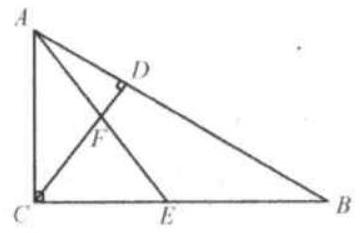
\includegraphics[width=\textwidth]{images/127(1).jpg}

\section*{Solution}
25/72.
Triangle \(A B C\) is a 5-12-13 right triangle, so \(A B=13\).\\
We can determine from similar triangles \(A D=\frac{25}{13}\) and\\
\(D B=\frac{144}{13}\).\\
\centering

\includegraphics[width=\textwidth]{images/134.jpg}

Draw \(E G / / F D\).\\
Since \(C E=E B, D G=B G=\frac{1}{2} \times \frac{144}{13}=\frac{72}{13}\).\\
Since triangle \(A F D\) is similar to triangle \(A E C\),\\
\(\frac{A F}{F E}=\frac{A D}{D G}=\frac{\frac{25}{\frac{13}{72}}}{13}=\frac{25}{72}\).

\end{document}
